In this chapter the process of loading individual maps will be explained.
This involves loading the map, encoded as an image in the PNG format, parsing values from this format, and finally placing tiles in the game world representing those values.
Maps are closely tied to the Mission System and Custom Content described in chapter \ref{chapter:modules:missions}.
As follows, this means it falls under requirements 3 and 6 in section \ref{gamedesign:selectionofgametype:importantstuff}.

\section{Tiling}
As explained previously, our game is a top-down 2D action game.
The top-down 2D aspect of it is important when we are to generate our maps.
A historical, and still prevalent technique for 2D games, is using a tiling approach for the layout of both the backdrop of the map and entities within it.
Several different approaches to tiling have been used in games, including squares, isometric and hexagonal tiles.
Figures~\ref{fig:civ-1_square},~\ref{fig:civ-2_iso}~and~\ref{fig:wesnoth_hex}
show examples of games using each of the mentioned techniques of tiling.

\begin{figure}[H]
    \centering
    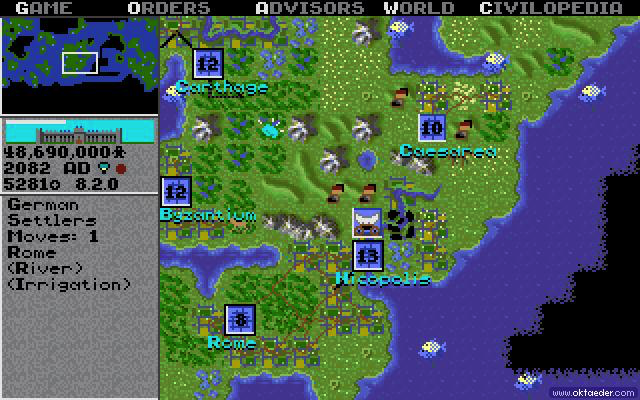
\includegraphics[width=0.7\textwidth]{figures/generating_levels/civ-1_square.png}
    \caption{Civilizations 1, using squares as tiles}\label{fig:civ-1_square}
\end{figure}

\begin{figure}[H]
    \centering
    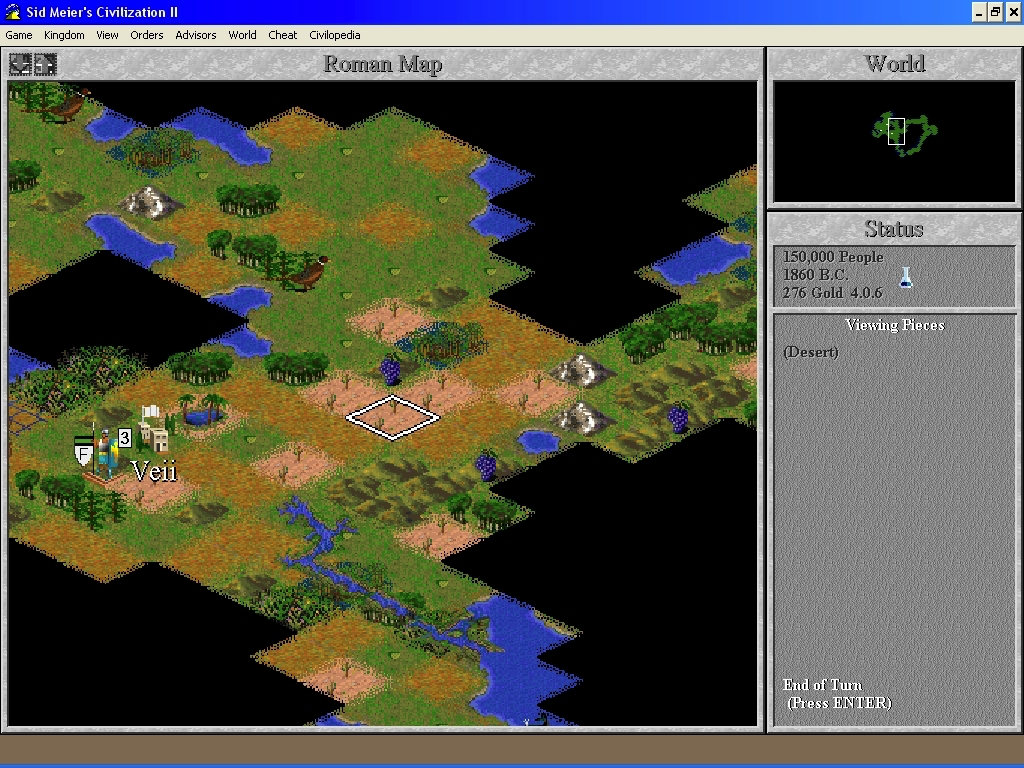
\includegraphics[width=0.7\textwidth]{figures/generating_levels/civ-2_iso.png}
    \caption{Civilizations 2, using the isometric technique}\label{fig:civ-2_iso}
\end{figure}

\begin{figure}[H]
    \centering
    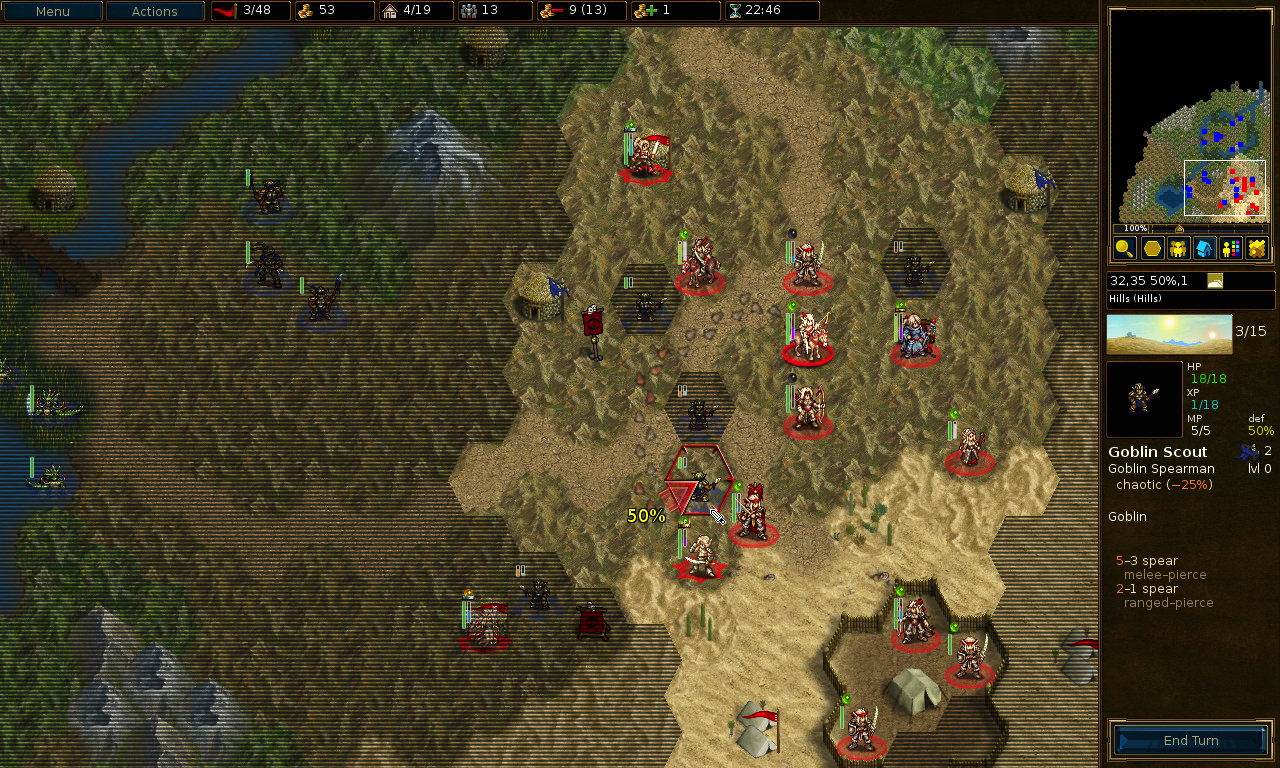
\includegraphics[width=0.7\textwidth]{figures/generating_levels/wesnoth_hex.png}
    \caption{Battle of Wesnoth, using a hexagonal tiling technique}\label{fig:wesnoth_hex}
\end{figure}
Since the individual techniques mostly impact the visual appearance of the game, the underlying data structures remain the same.
We have chosen to apply the most straightforward tiling technique: square tiles.

\section{Designing and loading maps}
Map creation is an important aspect when developing a game, and for this project there are different elements to consider for the map creation workflow.
\begin{itemize}
    \item The development process is agile, meaning the map should be easily modifiable to adapt to changes
    \item Game balancing, requiring the production of maps at a sufficient pace in order to quickly iterate on game balancing topics, such as strategies for a particular map layout
    \item The project has no dedicated map designer whom we can allocate to finely tune and manually design maps
\end{itemize}
These elements set up some different challenges to the project.
To keep up with potential changes, a quick way to create maps is preferred for the following reasons:
\begin{itemize}
    \item Designing maps and placing gameobjects in the Editor does not afford quick iterations, as required by our development process.
    \item The Editor does not afford easy refactoring of large maps, in that objects must be moved or replaced manually. \textit{Large} is relative, but for our purposes it could be upwards 100 gameobjects.
    \item Individual maps would have to reside in individual \texttt{Scene} files, increasing the complexity of collaboration since scenefiles do not  automatically merge correct in git, the version control system we use.
\end{itemize}

While there are different approaches for circumventing the above inconveniences, our solution is to encode the layout of each individual map in an external file which is then loaded and interpreted.
Historically, game developers have often used this approach, usually encoded in some in-house binary format~\cite{quake-bsp-format}.
While developing a custom format would offer significant flexibility, it would also result in additional development, especially with regards to players creating custom maps as a custom map editor would have to be designed and implemented.
Instead the choice of encoding the map in the PNG format was made, as described in section \ref{sec:modules:missions:customcontent}.
Using the PNG format, it is only a matter of specifying \textit{what} a particular color should encode and interpreting that color when loading a map.
As an example, the following could specify how colors could encode information about a map:
\begin{itemize}
    \item Black would be ground
    \item Green is grass
    \item Red is building floor
    \item And yellow being building walls
\end{itemize}
One obvious shortcoming from the above example is the lack of variation - maybe one would like to be able to specify different types of walls or floors. 
This could be mitigated by either specifying more colors or by interpreting a color differently depending on the context of the pixel.
To introduce variety into our maps, we use the latter approach for some colors, which we will describe later in this chapter.

Having decided on the format and encoded color values, we can design maps such as seen in figure~\ref{fig:png_map}.

\begin{figure}[H]
    \centering
    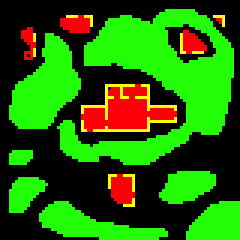
\includegraphics[width=0.7\textwidth]{figures/generating_levels/map.png}
    \caption{A PNG image encoding a map.}
    \label{fig:png_map}
\end{figure}
By looking at Figure~\ref{fig:png_map}, it is illustrated that there are some patches of grass, a building in the middle of the map and some torn-down buildings in the periphery of the map encoded in the PNG.
A single blue pixel encodes where the crafting table should be placed within the map.
\\\\
Color values can then separated into a new two-dimensional array, each cell consisting of the color value of its corresponding pixel, as illustrated on the right side in Figure \ref{fig:png_to_array}.
The data within that array is what we use to generate tiles and some game entities within the gameworld.
%thread carefully below...
%no
\begin{figure}[H]
    \centering
    \begin{tabular}{cc}
        {\footnotesize
            \setlength{\tabcolsep}{4.5pt}
            \begin{tabular}{|c|c|c|c|c|c|c|c|c|c|}
                \hline
                \cellcolor{black} & \cellcolor{black} & \cellcolor{black} &
                \cellcolor{black} & \cellcolor{black} & \cellcolor{red} &
                \cellcolor{red} & \cellcolor{red} & \cellcolor{red} &
                \cellcolor{red} \\ \hline
                \cellcolor{green} & \cellcolor{green} & \cellcolor{black} &
                \cellcolor{black} & \cellcolor{black} & \cellcolor{yellow} &
                \cellcolor{red} & \cellcolor{red} & \cellcolor{red} &
                \cellcolor{red} \\ \hline
                \cellcolor{green} & \cellcolor{green} & \cellcolor{green} &
                \cellcolor{black} & \cellcolor{black} & \cellcolor{yellow} &
                \cellcolor{red} & \cellcolor{red} & \cellcolor{red} &
                \cellcolor{red} \\ \hline
                \cellcolor{green} & \cellcolor{green} & \cellcolor{green} &
                \cellcolor{black} & \cellcolor{black} & \cellcolor{yellow} &
                \cellcolor{red} & \cellcolor{red} & \cellcolor{red} &
                \cellcolor{red} \\ \hline
                \cellcolor{green} & \cellcolor{green} & \cellcolor{green} &
                \cellcolor{black} & \cellcolor{black} & \cellcolor{yellow} &
                \cellcolor{yellow} & \cellcolor{red} & \cellcolor{red} &
                \cellcolor{yellow} \\ \hline
                \cellcolor{green} & \cellcolor{green} & \cellcolor{green} &
                \cellcolor{black} & \cellcolor{black} & \cellcolor{black} &
                \cellcolor{black} & \cellcolor{black} & \cellcolor{black} &
                \cellcolor{black} \\ \hline
                \cellcolor{green} & \cellcolor{green} & \cellcolor{green} &
                \cellcolor{green} & \cellcolor{black} & \cellcolor{black} &
                \cellcolor{black} & \cellcolor{black} & \cellcolor{black} &
                \cellcolor{black} \\ \hline
                \cellcolor{green} & \cellcolor{green} & \cellcolor{green} &
                \cellcolor{green} & \cellcolor{black} & \cellcolor{black} &
                \cellcolor{black} & \cellcolor{black} & \cellcolor{black} &
                \cellcolor{black} \\ \hline
                \cellcolor{green} & \cellcolor{green} & \cellcolor{green} &
                \cellcolor{green} & \cellcolor{green} & \cellcolor{black} &
                \cellcolor{black} & \cellcolor{black} & \cellcolor{black} &
                \cellcolor{black} \\ \hline
                \cellcolor{green} & \cellcolor{green} & \cellcolor{green} &
                \cellcolor{green} & \cellcolor{green} & \cellcolor{green} &
                \cellcolor{green} & \cellcolor{green} & \cellcolor{green} &
                \cellcolor{black} \\ \hline
            \end{tabular}
        }
        &
        {\footnotesize
            \setlength{\tabcolsep}{2.5pt}
            \begin{tabular}{|c|c|c|c|c|c|c|c|c|c|}
                \hline
                0 & 0 & 0 & 0 & 0 & 4 & 4 & 4 & 4 & 4 \\ \hline
                1 & 1 & 0 & 0 & 0 & 3 & 4 & 4 & 4 & 4 \\ \hline
                1 & 1 & 1 & 0 & 0 & 3 & 4 & 4 & 4 & 4 \\ \hline
                1 & 1 & 1 & 0 & 0 & 3 & 4 & 4 & 4 & 4 \\ \hline
                1 & 1 & 1 & 0 & 0 & 3 & 3 & 4 & 4 & 3 \\ \hline
                1 & 1 & 1 & 0 & 0 & 0 & 0 & 0 & 0 & 0 \\ \hline
                1 & 1 & 1 & 1 & 0 & 0 & 0 & 0 & 0 & 0 \\ \hline
                1 & 1 & 1 & 1 & 0 & 0 & 0 & 0 & 0 & 0 \\ \hline
                1 & 1 & 1 & 1 & 1 & 0 & 0 & 0 & 0 & 0 \\ \hline
                1 & 1 & 1 & 1 & 1 & 1 & 1 & 1 & 1 & 0 \\ \hline
            \end{tabular}
        }
    \end{tabular}
    \caption{Interpreting a PNG map image into a two-dimensional array}\label{fig:png_to_array} 
\end{figure}

\section{Implementation}
The implementation of generating backdrop tiles underwent several iterations
throughout the project and we explain some of the changes in this section.


The first naive implementation that we prototyped, was to iterate through the two-dimensional map and place tiles corresponding to the values, with tiles being \texttt{sprites} in the gameworld.
In Unity sprites need to be assigned a \texttt{sprite renderer} component which in turn needs to be attached a \texttt{gameobject}.
This effectively means that for each tile, an instantiation of a gameobject has
to be made, which can easily become expensive w.r.t to computation time.

Since tiles exhibit no particular behavior, it seems excessive to instantiate gameobjects for each tile.
This method also resulted in performance implications on mobile devices.
It is possible to substantially reduce the gameobjects required to be instantiated by \textit{grouping} similar areas into bigger tiles.
To do this, the map needs to be grouped such that large area consisting of only one type will be marked with a similar value in the data structure.
The groups are then \textit{blitted} together in a tile-pattern to form a larger texture.
There is a technical limit to this technique however, as texture-resolutions are limited by hardware, as such we limit the resolution of larger textures to $1024 \times 1024$.
Textures also preferably have to be square in dimensions due to technical
reasons such as compression optimizations on GPUs.
A comparison of the result of the two techniques can be seen in figure~\ref{fig:grouped_tiling_comparison}.
\begin{figure}[H]
    \centering
    \begin{tabular}{cc}
        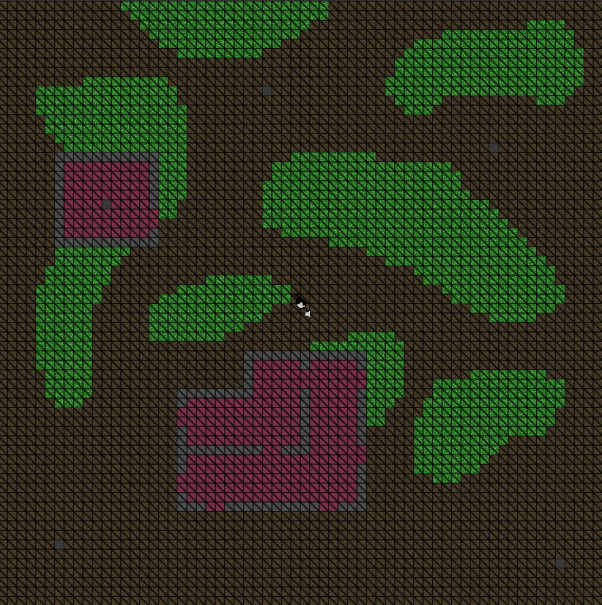
\includegraphics[width=0.5\textwidth]{figures/generating_levels/naive-tile.png}
        &
        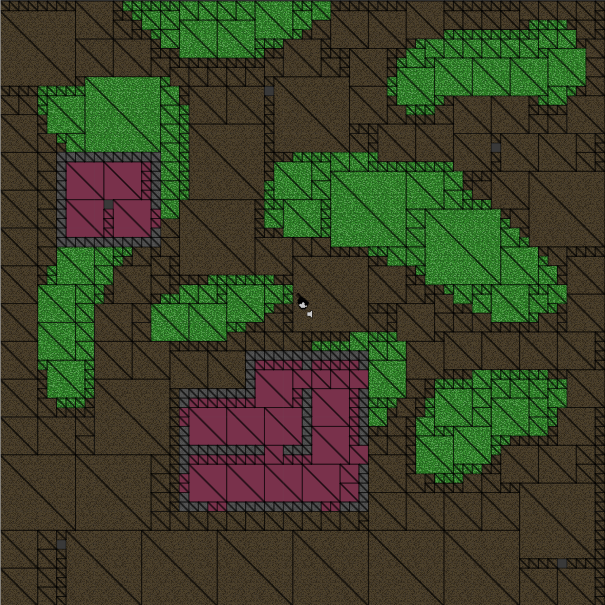
\includegraphics[width=0.5\textwidth]{figures/generating_levels/grouped-tile.png}
    \end{tabular}
    \caption{(left) naive tiling, (right) grouping tiles into larger tiles}\label{fig:grouped_tiling_comparison}
\end{figure}
The computation involved in blitting textures together \textit{can} be significant on mobile devices, as the larger textures have to be uploaded to the GPU in order to reflect changes.
The blitting is performed during runtime whenever a map is loaded, so in order to avoid blitting the same texture more than once, a caching of the larger textures to disk is performed, such that they can be loaded between subsequent runs of the application.
By caching and loading already blitted textures to disk, we significantly reduced loading times on mobile devices.\\

\textit{Transition} tiles between certain type of tiles, in particular between grass and ground, are desired.
This technique is also used in the games seen in figures~\ref{fig:civ-1_square},~\ref{fig:civ-2_iso}~and~\ref{fig:wesnoth_hex}.
To achieve this, an adaptation of the \textit{Marching squares} algorithm is used, and marks a position in the data structure as a particular type, based on the values of its neighbouring values~\cite{marching-squares}.
A corresponding \textit{transition tile} is then blitted together, cached to disk in the same manner as grouped tiles, and assigned to the gameobject at that position.
Figure~\ref{fig:transition_comparison} shows a comparison before and after integrating the algorithm.

\begin{figure}[H]
    \centering
    \begin{tabular}{cc}
        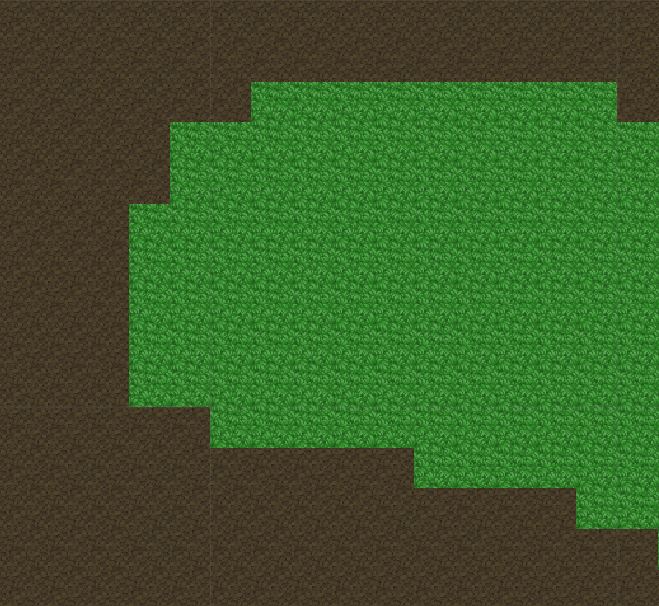
\includegraphics[width=0.5\textwidth]{figures/generating_levels/no_transition.png}
        &
        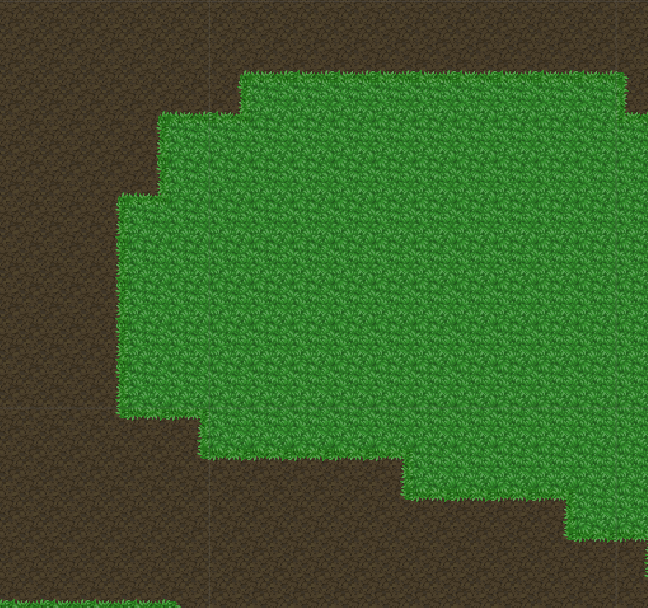
\includegraphics[width=0.5\textwidth]{figures/generating_levels/with_transition.png}
    \end{tabular}
    \caption{(left) without transitioning, (right) with transitioning tiles}\label{fig:transition_comparison}
\end{figure}

The final iteration generating tiles underwent brought with it additional
improvements w.r.t. to both loading and runtime. The improvement involves using
Unity3D's primitive \texttt{Quad} instead of \texttt{Sprite}. Although
Unity3D's documentation for \texttt{Sprite} describes it as graphical object
for use in 2D gameplay\cite{unitySprite}, for our purpose using a
\texttt{Quad} proved to be a better approach. Quads have the
capability of \textit{tiling} and \textit{shifting} its associated texture, and
especially being able to tile a texture is useful in our case. This enables us
to create rectangular areas of any size and eliminates the need for blitting
textures together into larger textures. We developed an algorithm for finding
rectangular areas on the map, which can be applied for each of the tile types
(grass, walls, etc.). In the case of ground tiles, we can scale a single quad
to cover the entire game-area, reducing the number of quads we need to
instantiate.

\begin{figure}[H]
    \centering
    \begin{tabular}{cc}
        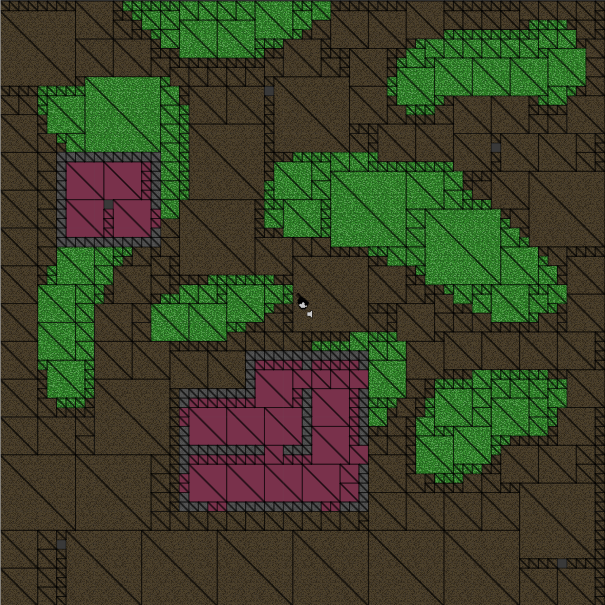
\includegraphics[width=0.5\textwidth]{figures/generating_levels/grouped-tile.png}
        &
        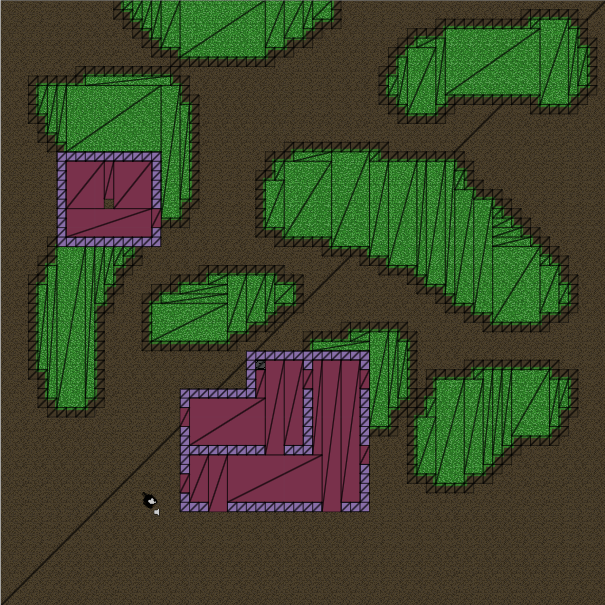
\includegraphics[width=0.5\textwidth]{figures/generating_levels/quad-tile.png}
    \end{tabular}
    \caption{(left) grouped tiling, (right) tiles using quads with tiled
    textures}\label{fig:quad_tiling_comparison}
\end{figure}

The iteration also brought with it a significant refactoring following a
functional style. This enabled us to divide the workload of finding rectangular
areas, amongst other things, to several separate threads. While this does not
guarantee improvements w.r.t. computation time, it has the potential to be an
improvement on multi-core platforms.

The difference in using quads instead of sprites can be seen
in Figure~\ref{fig:quad_tiling_comparison}


\section{Placing walls and colliders}
Placing walls involves both placing them as textured tiles within the gameworld, and placing \textit{colliders} such that moving object in the game cannot move through them.

\subsection{Placing wall sprites}
A naive implementation for placing wall-sprites within the gameworld is to place a gameobject with the texture of a wall.
However, the walls should fit seamlessly together as a homogeneous unit.
This is done using an adaptation of the \textit{Marching squares}, following the same procedure as with transitional tiles between grass and ground.
Firstly it is detected if a wall is a ``stump'', a regular vertical or horizontal middle section or a t-section. 
Diagonal walls are treated as ``stumps'', so our marching squares adaptation only considers adjacent tiles at 90-degree angles.
Figure~\ref{fig:wall_comparison} illustrates an example of placing walls where tiles are not ``connected'' and one where tiles are ``connected'' and figure~\ref{fig:walls_ingame} showing an in-game example.

\begin{figure}[H]
    \centering
    \begin{tabular}{cc}
        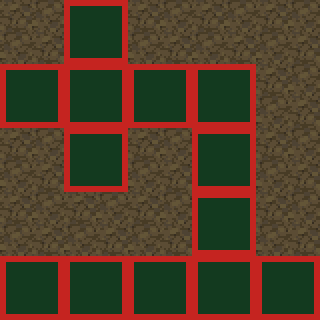
\includegraphics[width=0.5\textwidth]{figures/generating_levels/wall_no_border.png}
        &
        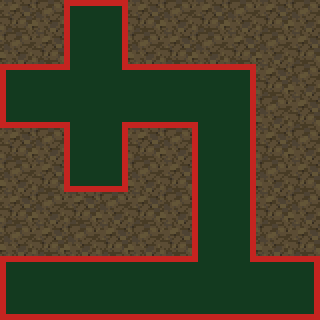
\includegraphics[width=0.5\textwidth]{figures/generating_levels/wall_with_border.png}
    \end{tabular}
    \caption{(left) not connected, and (right) where walls are connected}\label{fig:wall_comparison}
\end{figure}

\begin{figure}[H]
    \centering
    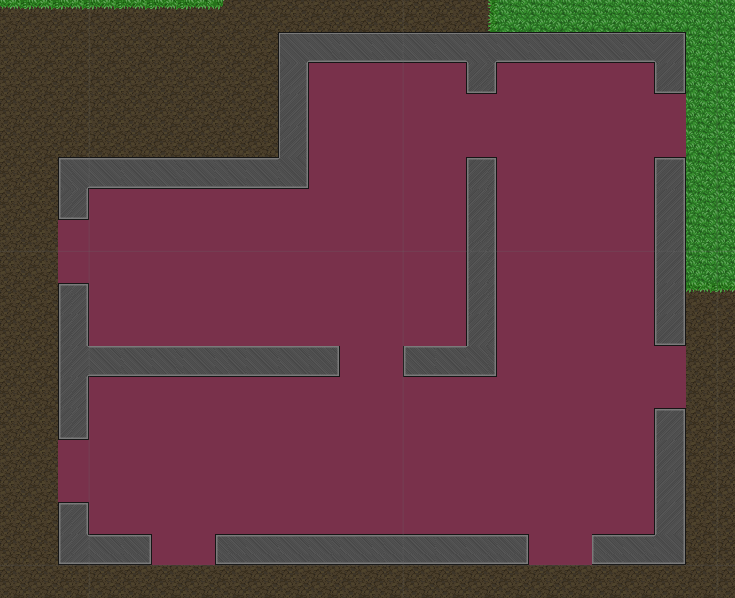
\includegraphics[width=\textwidth]{figures/generating_levels/walls_ingame.png}
    \caption{In-game example of connected walls}\label{fig:walls_ingame} 
\end{figure}

\subsection{Placing wall colliders}
For wall colliders it is desired to find the contour of walls and place gameobjects assigned a collide-able component in the gameworld inside the contour.
The first naive implementation is to place a square collider (regular \texttt{Collider2D}) for each wall tile.
An example of placing colliders at each wall tile can be seen in figure~\ref{fig:wall_with_vertices}.
This resulted in the unfortunate behaviour that collisions from rigidbodies - the player and enemies - behaved unreliable and rigid bodies would ``bounce off'' the walls whenever they would be ``between'' two collider sections.
\\
A solution to this problem is to place \texttt{Polygon Collider2D}s, using the contour vertices of the colliders shown in figure~\ref{fig:wall_with_vertices}. 
However this reveals another problem: the resulting polygon is concave.
This means that the polygon cannot \textit{easily} be constructed only knowing the vertices.
Our solution was to use an adaptation of \textit{flood fill} to first find connected vertical and then horizontal wall sections.
From the algorithm, we can find contour vertices for convex polygons which are \textit{larger} than single wall sections.
This significantly reduces the number of colliders necessary and eliminating the mentioned problem of unreliable behavior for rigidbodies colliding with walls.
An \textit{optimal} solution would be to construct a concave polygon from the vertices, which would require finding all contours \textit{and} the order in which they should connected when constructing the polygon.
The result of our \textit{flood fill} approach can be seen in figure~\ref{fig:wall_with_convex}.

\begin{figure}[H]
\centering
    \begin{minipage}{.4\textwidth}
    \centering
	    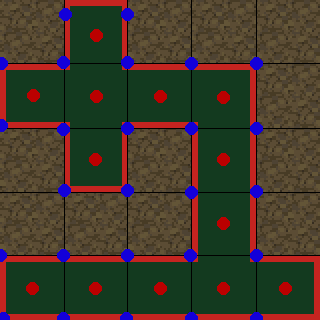
\includegraphics[scale=0.4]{figures/generating_levels/wall_with_vertices.png}
	    \captionof{figure}{Placing colliders at\\ tile positions.}\label{fig:wall_with_vertices} 
    \end{minipage}%
    \begin{minipage}{.4\textwidth}
    \centering
	    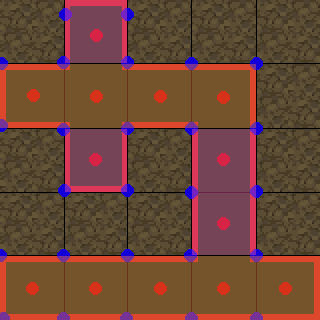
\includegraphics[scale=0.4]{figures/generating_levels/wall_with_convex.png}
   	    \captionof{figure}{Finding the connected convex polygons using flood fill.}\label{fig:wall_with_convex} 
    \end{minipage}
\end{figure}